%27/09 - Luis del Peso
\chapter{Modelos estadísticos en el análisis de secuencias}
\section{Secuencias biológicas como cadenas o strings}
El ADN, el ARN y las proteínas son responsables del almacenamiento, mantenimiento y ejecución de la información genética, representando así el dogma central de la biología molecular. Estas moléculas están compuestas por miles de átomos dispuestos en complejas estructuras tridimensionales. Y lo que es más importante, la estructura de estas moléculas es clave para su función. Una característica notable común a estas biomoléculas es que, a pesar de su complejidad estructural, son \textbf{polímeros lineales de un número limitado de subunidades (monómeros)} y un gran número de pruebas experimentales indican que la secuencia de los monómeros en la estructura lineal de estas moléculas es el principal determinante de sus propiedades, incluidas la estructura y la función. Así pues, estas moléculas pueden conceptualizarse como cadenas de símbolos y este sencillo modelo capta sus propiedades más fundamentales. Sorprendentemente, esta abstracción coincide con la definición formal de una cadena en las herramientas matemáticas y computacionales.

\subsection{Definición formal de una cadena}
En los lenguajes formales, como los utilizados en matemáticas e informática, una cadena se define como una secuencia finita de símbolos de un alfabeto determinado. Sea $\Sigma$ un conjunto finito no vacío de símbolos (caracteres), llamado alfabeto. Una cadena sobre $\Sigma$ es cualquier secuencia finita de símbolos de $\Sigma$. El número total de símbolos de una cadena s se conoce como longitud de secuencia, o simplemente longitud, y se suele representar como $||s||$. Una palabra suele ser una cadena sobre $\Sigma$ de longitud definida. El conjunto de todas las cadenas de longitud n sobre $\Sigma$, es decir, el conjunto de todas las palabras de tamaño n, se denomina $\Sigma^n$. Existen varias operaciones definidas para las cadenas, que también pueden representarse como nodos de un gráfico. En realidad, esto es clave para algunos métodos computacionales utilizados para ensamblar genomas completos a partir de estrategias de secuenciación shotgun.

\subsection{ADN como cadena}
Una molécula de ADN puede idealizarse como una cadena sobre el conjunto \{A, C, G, T\}, donde cada símbolo representa uno de los cuatro monómeros de nucleótidos del ADN, y una proteína como una cadena sobre el conjunto \{A, C, D, E, F, G, H, I, K, L, M, N, P, Q, R, S, T, V, W, Y\}, donde cada símbolo representa cada uno de los 20 residuos de aminoácidos (monómeros) presentes en las proteínas naturales. Si $\Sigma = \{A, C, G, T\}$, entonces $\Sigma^3$ representa los codones del código genético.

\section{Modelos estadísticos del ADN}
Consideremos que queremos construir un dispositivo (podría ser un programa informático o un artefacto físico como una ruleta, véase más adelante) que pueda producir una secuencia de ADN (es decir, una cadena sobre el conjunto \{A, C, G, T\}) que sea una cadena que tenga las mismas propiedades (composición y distribución de nucleótidos) que las moléculas de ADN reales. Para ello podemos utilizar dos modelos: el modelo multinomial y el modelo de cadena de Markov.

\subsection{Modelo multinomial}
El modelo más simple de secuencias de ADN asume que los nucleótidos son independientes e idénticamente distribuidos (iid), es decir, la secuencia ha sido generada por un proceso que produce cualquiera de los cuatro símbolos en cada posición de secuencia i al azar, extrayéndolos independientemente de la misma distribución de probabilidad \footnote{Una distribución de probabilidad es una lista de los posibles resultados con sus correspondientes probabilidades que cumple tres reglas: 1. los resultados deben ser disjuntos; 2. cada probabilidad debe estar comprendida entre 0 y 1; 3. las probabilidades deben sumar 1.} sobre el alfabeto \{A, C, G, T\}.

Se puede generar una secuencia de ADN según el modelo multinomial \footnote{La distribución binomial describe la probabilidad de obtener un número determinado de éxitos en n experimentos independientes. Fundamentalmente, la distribución binomial se aplica sólo cuando el experimento tiene sólo dos resultados posibles. La distribución multinomial es una generalización de la distribución binomial donde cada variable aleatoria puede tomar más de dos valores.} utilizando un dispositivo sencillo como el que se representa en la figura \ref{fig:ruletas}. El modelo de secuencia multinomial es como tener una ruleta que se divide en cuatro partes diferentes etiquetadas como A, T, G y C, donde pA, pT, pG y pC son las fracciones de la ruleta ocupadas por los cortes con estas cuatro etiquetas. Si se hace girar la flecha situada en el centro de la rueda de la ruleta, la probabilidad de que se detenga en la porción con una etiqueta particular (por ejemplo, la porción etiquetada como "A") solo depende de la fracción de la rueda ocupada por esa porción (pA aquí).

\begin{figure}[htbp]
\centering
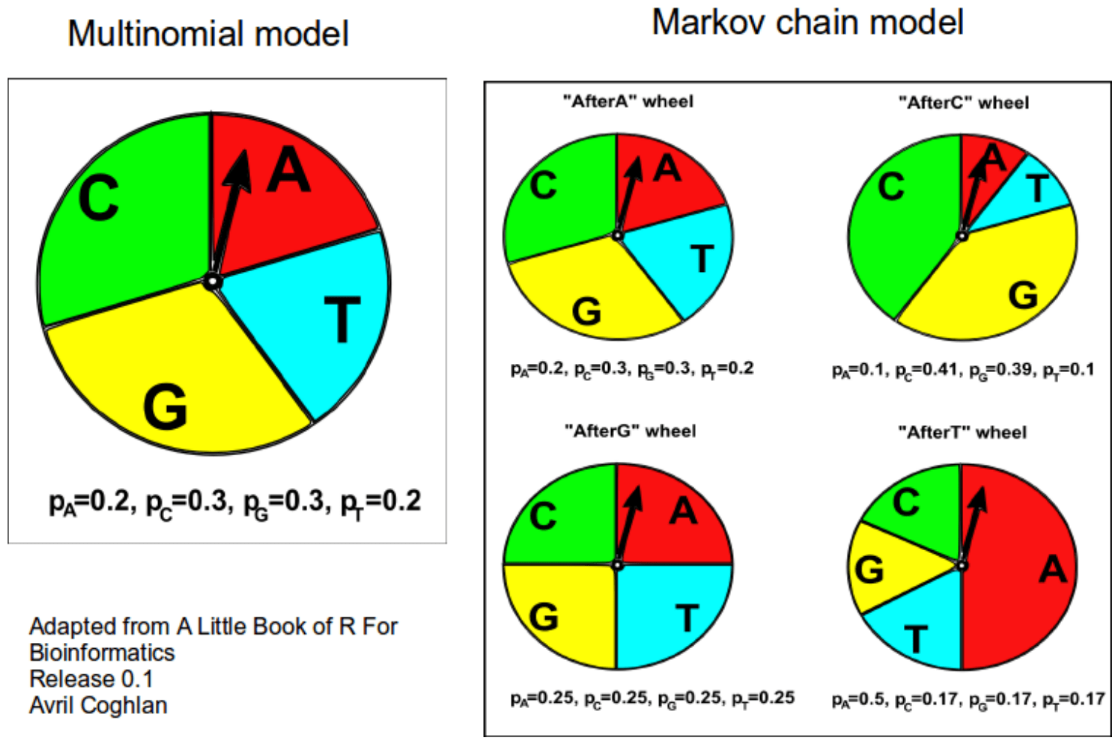
\includegraphics[width = 0.55\textwidth]{figs/ruletas.png}
\caption{Comparación de los modelos de secuencia de ADN multinomial y cadena de Markov. }
\label{fig:ruletas}
\end{figure}

En una cadena generada por un modelo multinomial, la probabilidad de observar el símbolo (nucleótido en el caso del ADN y aminoácido en el caso de la proteína) x en la posición i de la secuencia se denota por $p_x,i = p(s(i)=x)$ y no depende de la posición i. Por lo tanto, podemos calcular la probabilidad de observar la cadena s donde n = ||s|| como:

 $$ p(s) = \prod_{i=1}^{n} p(s_i) $$

\textit{Ejemplo práctico:}
En un experimento ChIP-seq (una técnica de secuenciación masiva que permite identificar sitios de unión de proteínas al ADN), se descubrieron 500 sitios de unión para un factor de transcripción. Dado que el genoma humano contiene entre 20,000 y 26,000 genes, estos 500 sitios pueden parecer pocos. Sin embargo, la cuestión central es si esta cantidad es coherente con lo que se esperaría bajo un modelo estadístico.
Los factores de transcripción se unen a subsecuencias específicas de ADN llamadas "motivos de respuesta". En este caso, el motivo de unión es RCGTG, donde R representa A o G. Aunque las moléculas biológicas interaccionan con cierta flexibilidad, este motivo es bastante restringido, ya que solo una posición es flexible. El genoma humano tiene alrededor de $3 \times 10^9$ bases, por lo que podemos calcular la cantidad esperada de sitios de unión basándonos en la probabilidad de que este motivo ocurra aleatoriamente.
Asumiendo que los nucleótidos son independientes entre sí y tienen la misma probabilidad de aparecer, la probabilidad de que aparezca la secuencia CGTG es $0,25^4$. Para la posición R, que puede ser A o G, la probabilidad es $0,5$. Por tanto, la probabilidad total de encontrar el motivo RCGTG es $0,25^4 \times 0,5 = \frac{1}{512}$, es decir, se esperaría encontrar esta secuencia una vez cada 512 posiciones. Con un genoma de $3 \times 10^9$ bases, se esperaría aproximadamente $\frac{3 \times 10^9}{512} \approx 6 \times 10^6$ sitios. Sin embargo, en el experimento solo se hallaron 500 sitios, lo que sugiere que el modelo experimental no refleja completamente la realidad biológica y es necesario recurrir a otros modelos, aunque sean simplificados.
La secuencia por sí sola no es suficiente para que el factor de transcripción se una. Otros factores, como la accesibilidad de la cromatina, también juegan un papel crucial. No obstante, el modelo multinomial proporciona una referencia útil para evaluar los datos experimentales en un contexto aleatorio.
Si bien este enfoque es sencillo, tiene limitaciones significativas, como la suposición de independencia entre nucleótidos. Sabemos que esto no es siempre cierto, por ejemplo, los dinucleótidos CG suelen ser menos frecuentes salvo en las "islas CpG", donde existe una gran concentración.

\subsubsection{Frecuencia de dinucleótidos}
Los dinucleótidos, que representan todas las combinaciones posibles de dos nucleótidos ($\Sigma^2$), deberían tener una frecuencia esperada de $\frac{1}{16}$ en el genoma humano. Al analizar las frecuencias observadas en el cromosoma 21, se encuentra que A y T aparecen con una frecuencia del 29.5\%, mientras que G y C con un 20.5\% (Figura \ref{fig:dinucleotidos}). Al recalcular las frecuencias de los dinucleótidos, se observa que, en general, la frecuencia observada coincide con la esperada, excepto para el dinucleótido CG, cuya frecuencia observada es tres veces menor a la esperada. Esto sugiere que los nucleótidos no son completamente independientes, y el modelo multinomial no es suficiente para describir esta dependencia.

\begin{figure}[htbp]
\centering
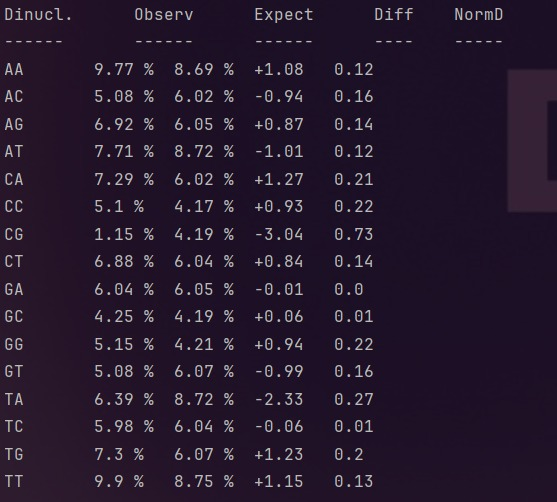
\includegraphics[width = 0.55\textwidth]{figs/freqs-dinucleotidos.jpg}
\caption{Cálculo de las frecuencias de los 16 dinucleótidos en el cromosoma 21 del ser humano. Los valores esperados y observados suelen coincidir en $\pm$ 1\% a excepción del dinucleótido CG. }
\label{fig:dinucleotidos}
\end{figure}
 
\subsection{Cadena de Markov}
El modelo multinomial es una herramienta sencilla e intuitiva que representa con precisión muchas secuencias biológicas de ADN. Sin embargo, se supone que la probabilidad de que aparezca un nucleótido en una posición determinada es independiente de la identidad de los residuos cercanos, lo que no siempre es así. Por ejemplo, si quisiéramos modelar un tramo de ADN que comprende una isla CpG, la probabilidad de observar una G estaría estrictamente condicionada a la identidad del residuo anterior, es decir, la probabilidad de observar una G después de una C sería probablemente más alta que después de cualquier otro residuo de nucleótido. Las cadenas de Markov pueden modelar correlaciones locales entre símbolos en una cadena. Para ello utilizan probabilidades condicionales. Por lo tanto, mientras que en el modelo multinomial se suponía que pG era constante a lo largo de la secuencia, en el modelo de cadena de Markov pG después de C $p(G|C)$ no es necesariamente igual a pG después de A $p(G|A)$.
Se puede generar una secuencia de ADN según el modelo de Markov utilizando un dispositivo sencillo como el que se muestra a la derecha en las figuras \ref{fig:ruletas} y \ref{fig:markov}. En este caso tenemos cuatro ruletas, cada una de las cuales representa las probabilidades de los nucleótidos del ADN. Para generar un residuo en cualquier posición determinada usando este modelo, elegiríamos una de estas cuatro ruedas de ruleta dependiendo del residuo que obtuviéramos en la posición anterior. Se podría representar todas estas probabilidades usando una matriz donde las filas representan el nucleótido encontrado en la posición anterior de la secuencia, mientras que las columnas representan los nucleótidos que podrían encontrarse en la posición actual de la secuencia. En la tabla \ref{tab:matrix} se muestra una representación de la ruleta a la derecha de la figura \ref{fig:ruletas} en forma de matriz.

\begin{table}[htbp]
    \centering
    \begin{tabularx}{\textwidth}{ X | X X X X}
          & To A & To C & To G & To T \\ \hline
         From A & 0,20 & 0,30 & 0,30 & 0,20 \\
         From C & 0,10 & 0,41 & 0,39 & 0,10 \\
         From G & 0,25 & 0,25 & 0,25 & 0,25 \\
         From T & 0,50 & 0,17 & 0,17 & 0,17 \\
    \end{tabularx}
    \caption{Matriz de transición de cadena de Markov.}
    \label{tab:matrix}
\end{table}

En la jerga de los modelos de Markov, esta matriz se denomina \textbf{matriz de transición}. La razón es que una cadena de Markov generadora de secuencia de ADN se puede idealizar como una estructura con cuatro estados diferentes, que representan cada uno de los cuatro nucleótidos, y la secuencia se produce por la transición de un estado a otro. Las transiciones entre estados no son igualmente probables, sino que ocurren con las probabilidades indicadas en los bordes que unen cada estado, que en conjunto son las probabilidades de transición y pueden representarse como una matriz de transición (véase figura \ref{fig:markov}).
Las entradas en la matriz de transición corresponden a probabilidades condicionales. Por ejemplo, pCG es la probabilidad de G en la posición i dado que hay una C en la posición i-1, es decir $pG = p(s_i = G|s_{i-1} = C)$. Por tanto, la probabilidad de la secuencia s según este modelo podría calcularse como $ p(s) = \prod p(s_i | s_{i-1}) $. Sin embargo, vale la pena señalar que, para representar una molécula de ADN lineal, también necesitaríamos un conjunto de parámetros que representen las probabilidades del primer nucleótido en la secuencia (dado que no hay uno anterior, podríamos obtener esta probabilidad de la matriz de transición). Si definimos estas probabilidades iniciales como $\pi(A), \pi(C), \pi(G), \pi(T)$, entonces la probabilidad de una secuencia lineal según este modelo se puede calcular como:

 $$ p(s) = \pi(s_1) * \prod_{i=2}^{n} p(s_i | s_{i-1}) $$
 
\begin{figure}[htbp]
\centering
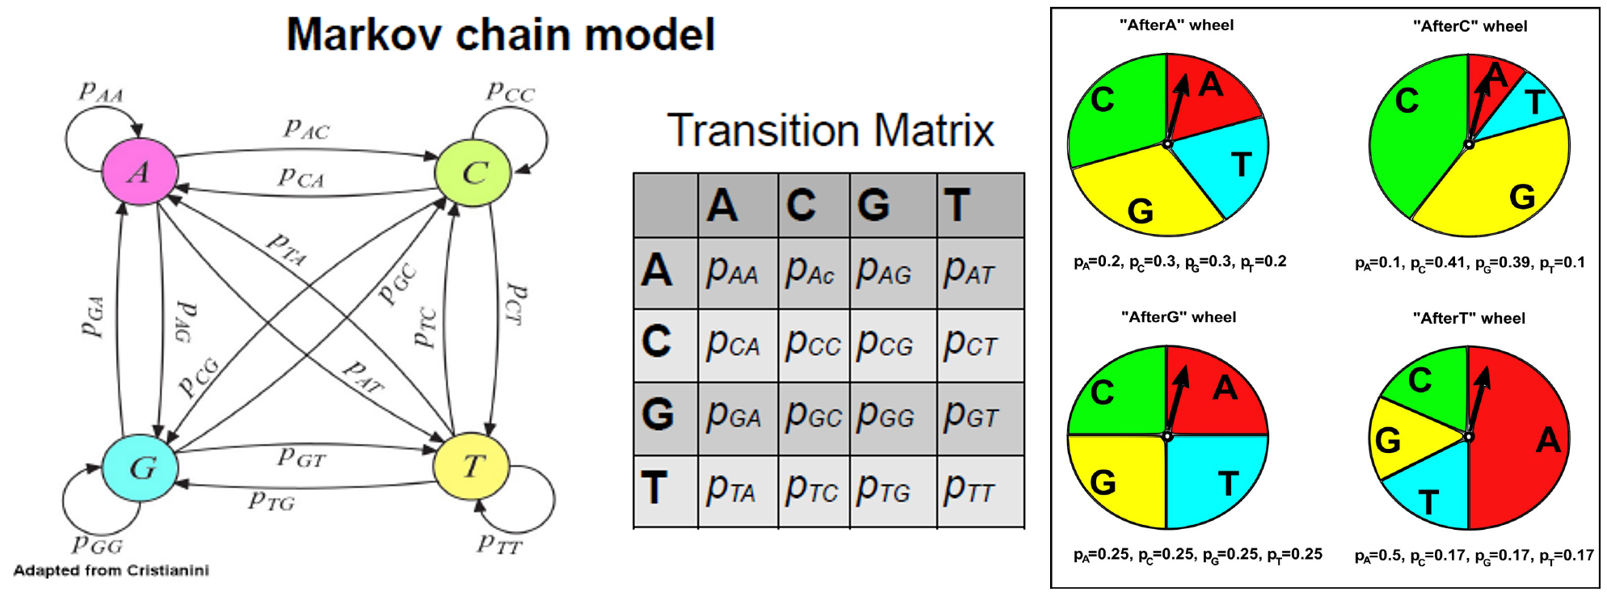
\includegraphics[width = 0.7\textwidth]{figs/markov.png}
\caption{Representaciones gráficas de la cadena de Markov. En la matriz de transición, las filas corresponden a los nucleótidos de la posición anterior y las columnas los nucleótidos que les siguen. }
\label{fig:markov}
\end{figure}
 
Por ejemplo, para calcular la probabilidad de encontrar la secuencia RCGTG utilizando este modelo, se deben considerar las probabilidades condicionales para cada posible combinación de nucleótidos. La probabilidad se calcula dividiendo la secuencia en dos casos, que luego se suman:
\begin{align*}
0,25 \times 0,3 \times 0,39 \times 0,25 \times 0,17 (ACGTG) \\
+ 0,25 \times 0,25 \times 0,39 \times 0,25 \times 0,17 (GCGTG) \\
= 0,001243 + 0,001036 \\
= 0,002279 
\end{align*}
 
\subsection{Ejercicios}
\textit{\textbf{Ejercicio 1:} 
Supongamos que el ADN humano puede dividirse en sólo dos tipos de regiones las ricas en C+G y el resto del ADN con una composición de bases no sesgada (no ricas en C+G). Suponiendo el modelo de independencia (la probabilidad de cada nucleótido en una posición dada es independiente de la identidad de los nucleótidos adyacentes) y que la secuencia es homogénea dentro de cada una de estas dos regiones, podemos representarlas mediante un modelo probabilístico multinomial. La región rica en G+C se define por los parámetros: pT=1/8, pC=3/8,pA=1/8 y pG=3/8. El resto del ADN por pT=pC=pA=pG=1/4. ¿Cuál es la probabilidad de observar la secuencia seg=CGACGCGCGCGTCG en una región rica en C+G? ¿Y en la no rica en G+C? Ahora bien, imaginemos que sólo el 1\% (¡me lo acabo de inventar!) del genoma es rico en C+G. Si tomamos un genoma de 14 pb al azar y resulta ser la secuencia CGACGCGCGCGTCG, ¿cuál sería la probabilidad de que proceda de una región rica en C+G?}
\begin{itemize}
\item Paso 1: Probabilidad de observar la secuencia en la región rica en C+G

La probabilidad de observar una secuencia en una región rica en C+G, dada la independencia entre los nucleótidos, es el producto de las probabilidades de cada nucleótido en la secuencia. Las probabilidades en la región rica en C+G son las siguientes:

\[
p_T = \frac{1}{8}, \quad p_C = \frac{3}{8}, \quad p_A = \frac{1}{8}, \quad p_G = \frac{3}{8}
\]

Dada la secuencia \texttt{CGACGCGCGCGTCG}, la probabilidad de observarla en la región rica en C+G es:

\[
P(\text{CGACGCGCGCGTCG} \mid \text{C+G}) = p_C \cdot p_G \cdot p_A \cdot p_C \cdot p_G \cdot p_C \cdot p_G \cdot p_C \cdot p_G \cdot p_C \cdot p_G \cdot p_T \cdot p_C \cdot p_G
\]

Sustituyendo los valores de las probabilidades:

\small
\[
P(\text{CGACGCGCGCGTCG} \mid \text{C+G}) = 
\]

\[
\left( \frac{3}{8} \right) \cdot \left( \frac{3}{8} \right) \cdot \left( \frac{1}{8} \right) \cdot \left( \frac{3}{8} \right) \cdot \left( \frac{3}{8} \right) \cdot \left( \frac{3}{8} \right) \cdot \left( \frac{3}{8} \right) \cdot \left( \frac{3}{8} \right) \cdot \left( \frac{3}{8} \right) \cdot \left( \frac{3}{8} \right) \cdot \left( \frac{3}{8} \right) \cdot \left( \frac{1}{8} \right) \cdot \left( \frac{3}{8} \right) \cdot \left( \frac{3}{8} \right)
\]

\[
= 1,2 \cdot 10^{-7}
\]

\normalsize

\item Paso 2: Probabilidad de observar la secuencia en la región no rica en C+G

En la región no rica en C+G, las probabilidades de cada nucleótido son iguales:

\[
p_T = p_C = p_A = p_G = \frac{1}{4}
\]

Por lo tanto, la probabilidad de observar la secuencia \texttt{CGACGCGCGCGTCG} es:

\[
P(\text{CGACGCGCGCGTCG} \mid \text{no C+G}) = \left( \frac{1}{4} \right)^{14} = 3,7 \cdot 10^{-9}
\]

\item Paso 3: Probabilidad de que la secuencia provenga de una región rica en C+G

Utilizamos el teorema de Bayes para calcular la probabilidad de que la secuencia provenga de una región rica en C+G. La fórmula de Bayes es:

\[
P(\text{C+G} \mid \text{secuencia}) = \frac{P(\text{secuencia} \mid \text{C+G}) \cdot P(\text{C+G})}{P(\text{secuencia})}
\]

Donde:
\begin{itemize}
\item $ P(\text{secuencia} \mid \text{C+G}) $ es la probabilidad de observar la secuencia en una región rica en C+G (calculada en el Paso 1).
\item $ P(\text{C+G}) = 0,01 $ es la proporción del genoma que es rico en C+G.
\item $ P(\text{secuencia}) $ es la probabilidad total de observar la secuencia, que se calcula como:
\end{itemize}

\[
P(\text{secuencia}) = P(\text{secuencia} \mid \text{C+G}) \cdot P(\text{C+G}) + P(\text{secuencia} \mid \text{no C+G}) \cdot P(\text{no C+G})
\]

Donde $ P(\text{no C+G}) = 1 - P(\text{C+G}) = 0,99 $

Sustituyendo todos los valores, podemos obtener la probabilidad de que la secuencia provenga de una región rica en C+G.

\[
\frac{1,2 \cdot 10^{-7} \cdot 0,01}{1,2 \cdot 10^{-7} \cdot 0,01 + 3,7 \cdot 10^{-9} \cdot 0,99} = 0,25
\]

\end{itemize}

\textit{\textbf{Ejercicio 2:} 
Ha secuenciado un fragmento de la cadena + de un nuevo organismo. Nosotros suponemos que es un fragmento representativo y que la composición es homogénea en todo el genoma. Las frecuencias absolutas de bases en este fragmento de secuencia se indican en la tabla siguiente. Estima los siguientes parámetros de un modelo de cadena de Markov para esta secuencia. ¿Qué sería la probabilidad de transición de T a A (PTA) y la probabilidad de y la probabilidad de transición de A a A (PAA)? ¿Cuál sería la probabilidad PTA para el modelo de cadena de Markov de la cadena - de este dsADN? ¿Y la probabilidad de transición de transición PAA de la cadena -?}
\begin{table}[htbp]
    \centering
    \begin{tabularx}{\textwidth}{ X | X X X X}
          & To A & To C & To G & To T \\ \hline
         From A & 15 & 23 & 25 & 11 \\
         From C & 9 & 38 & 35 & 8 \\
         From G & 26 & 21 & 18 & 24 \\
         From T & 25 & 8 & 10 & 3 \\
    \end{tabularx}
\end{table}
Teniendo en cuenta las siguientes probabilidades condicionales:
$$P_{TA+} = \frac{25}{25 + 8 + 10 + 3} = 0,54 $$
$$P_{AA+} = \frac{15}{15 + 23 + 25 + 11} = 0,20 $$

En cuanto a la probabilidad de la cadena negativa, hay que tener en cuenta que las frecuencias están dadas en la cadena positiva. Por tanto, cuando se tiene en cuenta el cambio del segundo nucleótido de la pareja en la cadena negativa, el cambio en la cadena positiva se produce en el primero. \\

\begin{table}[htbp]
\centering
5' -----------TA-----------3' \\
3' -----------AT-----------5' \\
\end{table}

$$P_{TA-} = \frac{25}{25 + 15 + 26 + 9} = 0,33 $$

$$P_{AA-} = \frac{3}{3 + 24 + 8 + 11} = 0,065 $$

\subsection{Problema práctico: islas CpG}
Un desafío interesante sería escribir un programa que identifique islas CpG en un fragmento del genoma humano. Los dinucleótidos CG tienden a perderse debido a la metilación de la citosina, que, al desaminarse, se convierte en timina en lugar de regresar a citosina. Sin embargo, en regiones del genoma que no se metilan, como las regiones transcripcionalmente activas, las secuencias CG permanecen intactas, formando las llamadas islas CpG. El objetivo del programa sería localizar el inicio y el final de una de estas islas en una secuencia genómica. La isla CpG tiene una longitud de 1.000 bases, mientras que la región genómica tendrá aproximadamente unos 40.000 nucleótidos.

\begin{figure}[htbp]
\centering
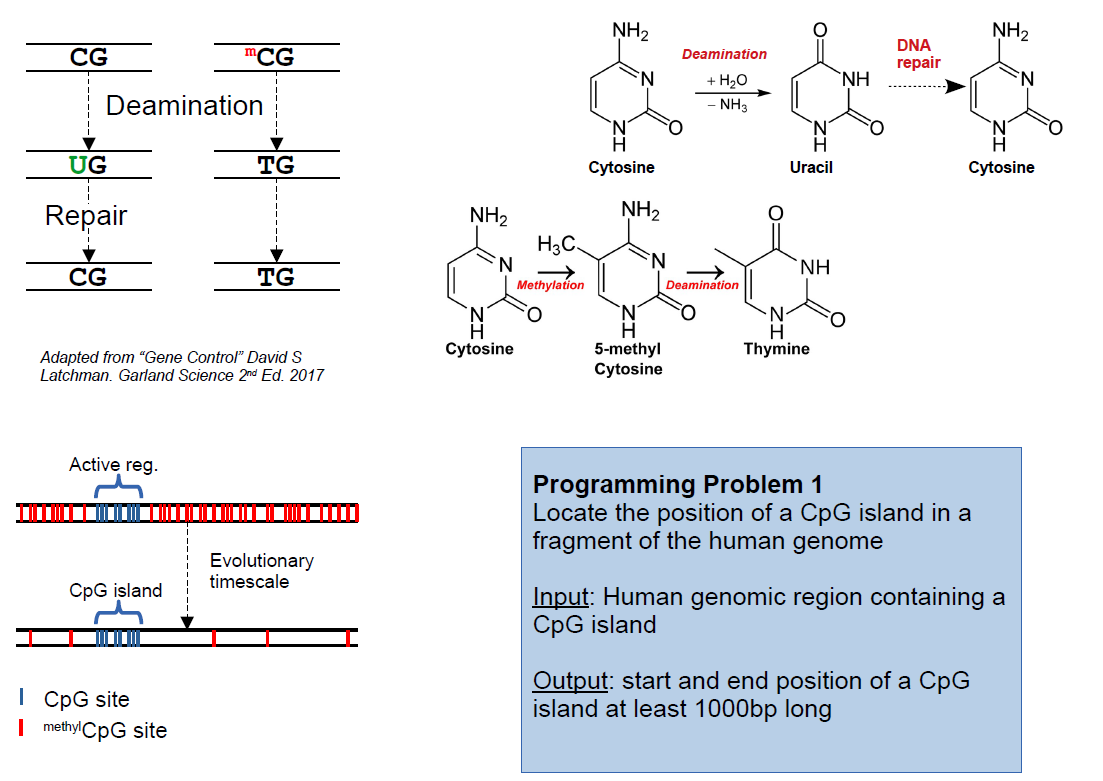
\includegraphics[width = 0.7\textwidth]{figs/cpg-islands.png}
\caption{Explicación biológica gráfica de las islas CpG. }
\end{figure}

Las islas CpG tienen una alta densidad de dinucleótidos de CG. Por tanto, hay que buscar una región genómica que tenga una alta densidad y que permita identificar la isla. Para ello, se debe emplear un sliding window, es decir, una ventana de una cierta cantidad de nucleótidos para calcular su frecuencia de CG. Como la isla CpG va a tener un tamaño de 1000, el tamaño razonable de ventana sería de 1000, y esta ventana se irá desplazando de nucleótido en nucleótido. En un gráfico que muestre la densidad de CG, se observaría una frecuencia muy superior (un pico alto) donde se encuentre la isla. Como la gráfica real es algo ruidosa, hay que establecer un threshold para poder obtener la posición concreta de la isla. Se puede utilizar la frecuencia total de CG en la secuencia (contabilizar todas las apariciones de CG y dividir por la longitud para obtener la media), pero hay que tener en cuenta el margen de error. Se puede calcular el porcentaje de CG en todas las ventanas, calcular la media y la desviación estándar para poder tener la dispersión esperada de una ventana concreta. Una vez con eso, se puede dibujar la distribución de los porcentajes de CpG para poder establecer la frecuencia de fondo de los dinucleótidos y separarla de la frecuencia de las islas CpG. En caso de una distribución normal, se pueden establecer criterios arbitrarios como los criterios estadísticos del 5\% superior (one value t-test). Esto resulta en una distribución empírica, pero se puede utilizar una distribución binomial para obtener el mismo resultado más formalmente correcto. También se puede aproximar a una distribución de Poisson para cada ventana. La forma más correcta sería mediante los modelos ocultos de Markov, teniendo como etiquetas que una posición pertenezca o no a una isla CpG. Esto se verá más adelante en la asignatura. 
